\documentclass{article}
\usepackage[utf8]{inputenc}
\usepackage{amssymb}
\usepackage{graphicx}
\graphicspath{ {./images/} }

\title{Regularization}
\author{Rishit Dagli}
\date{April 2020}

\begin{document}

\maketitle
\section{Cover image}
\vspace{5}

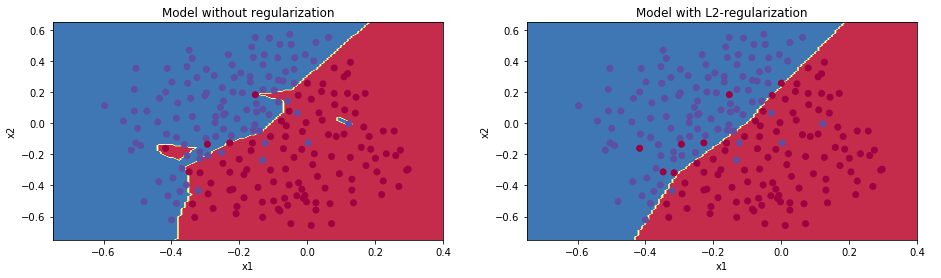
\includegraphics[width=\textwidth]{cover.png}

\maketitle
\section{Introduction}

Overfitting is a huge problem, specially in deep neural networks. If you suspect your neural network is over fitting your data .There are quite some methods to figure out that you are overfitting the data, maybe you have a high variance problem or you draw a train and test accuracy plot and figure out that you are overfitting. One of the first things you should try out probably in this case is regularization.

\maketitle
\section{Why Regularization?}

The other way to address high variance, is to get more training data that is quite reliable. If you get some more training data, you can think of it in this manner that you are trying to generalize your weights for all situations. And that solves the problem most of the time, so why anything else? But a huge downside with this is that you can not always get more training data, it could be expensive to get more data and sometimes it just could not be accessible.
\vspace{5}

It now makes sense for us to discuss about some method which would help us reduce overfitting. Adding regularization will often help to prevent overfitting. Guess what, there is a hidden benefit with this, often regularization also helps you minimize random errors in your network. Having discussed why the idea of regularization makes sense, let us now understand it.

\maketitle
\section{Understanding $L_2$ Regularization?}

We will start by developing these ideas for the logistic function. So just recall that you are trying to minimize a function J called the cost function which looks like this-

$$J = \frac{1}{m} \sum_{i=1}^m L(\hat{y^{(i)}}, y^{(i)})$$
Where $w \in \mathbb{R}^{n_x}$ and $b \in \mathbb{R}$

And your $w$ is a matrix of size $x$ and $L$ is the loss function. Just a quick refresher, nothing new.

So, to add regularization for this we will add a term to this cost function equation, we will see more of this-

$$\frac{\lambda}{2m}||w||^2_2$$

So $\lambda$ is another hyper parameter that you might have to tune, and is called the regularization parameter.

According to the ideal convention $||w||^2_2$ just means the Euclidean $L_2$ norm of $w$ and then just square it, let us summarise this in an equation so it becomes easy for us, we will just simplify the $L_2$ norm term a bit-

$$||w||^2_2 = \sum_{j=1}^{n_x} w_j^2 = w^Tw$$

I have just expressed it in the terms of the squared euclidean norm of the vector prime to vector $w$. So the term we just talked about is called $L_2$ regularization. Don't worry, we will discuss more about how we got the $\lambda$ term in a while but at least you now now have a rough idea of how it works. There is actually a reason of this method called "$L_2$ normalization", it is just called so because we are computing the $L_2$ norm of $w$

Till now, we discussed about regularization of the parameter $w$, and you might have asked yourself a question, why only $w$? Why not add a term with $b$? And that is a logical question. It turns out in practice you could add a $w$ term or do it for w but we usually just omit it. Because if you look at the parameters, you would notice that w is usually a pretty high dimensional vector and particularly has a high variance problem. Understand it as w just has a lot of individual parameters, so you aren't fitting all the parameters well, whereas $b$ is just a single number. So almost all of your major parameters are in w rather than in $b$. So, even if you add that last b term to your equation, in practice it would not make a great difference.

\maketitle
\section{$L_1$ Regularization?}

We just discussed about $L_2$ regularization and you might also have heard of $L_1$ regularization. So $L_1$ regularization is when instead of the term we were earlier talking about you just add L₁ norm of the parameter vector $w$. Let's see this term in a mathematical way-

$$\frac{\lambda}{2m} \sum_{i=1}^{n_x} |w| = \frac{\lambda}{2m} ||w||_1$$

\maketitle
\section{Extending the idea to Neural Nets}

We just saw how we would do regularization for the logistic function and you now have a clear idea of what regularization means and how it works. So, now it would be good to see how these ideas can extend to neural nets. So, recall or cost function for a neural net, it looks something like this-

$$J(w^{[1]}, b^{[1]}, w^{[2]}, b^{[2]} ... w^{[n]}, b^{[n]}) = \frac{1}{m}\sum^m_{i=1} L(\hat{y^{(i)}}, y^{(i)})$$

So, now recall what we added to this while we were discussing this earlier we added the regularization parameter $\lambda$, a scaling parameter and most importantly the $L_2$ norm so we will do something similar instead we will just sum it for the layers. So, the term we add would look like this-

$$\frac{\lambda}{2m} \sum_{l=1}^L ||w^{[l]}||^2$$

Let us now simplify this $L_2$$ norm term for us, it is defined as the sum of the $i$ over sum of $j$, of each of the elements of that matrix, squared-

$$||w^{[l]}||^2 = \sum^{n[l]}_{i=1} \sum^{n[l-1]}_{j=1} (w_{ij}^{[l]})^2$$

where $w: \hspace{1}(n^{[l]}, n^{[l-1]})$

What the second line here tells you is that your weight matrix or $w$ here is of the dimensions $n^l$, $n^{l-1}$ and these are the number of units in layer $l$ and $l-14 respectively. This is also called the "Frobenius norm" of a matrix, Frobenius norm is highly useful and is used in a quite a lot of applications the most exciting of which is in recommendation systems. Conventionally it is denoted by a subscript "F". You might just say that it is more easy to call it just L₂ norm but due to some conventional reasons we call it Frobenius norm and has a different representation-

$||\cdot||^2_2$ -L_2$$ norm
$||\cdot||^2_F$ - Frobenius norm

\maketitle
\section{Implementing Gradient Descent}

So, earlier when we would do is compute $dw$ using back propagation, get the partial derivative of your cost function $J$ with respect to w for any given layer l and then you just update you $w^1$ and also include the α parameter. Now that we have got our regularization term into our objective, so we will simply add a term for the regularization-

$$dw^{[l]} = (from \hspace{5} backprop.) + \frac{\lambda}{m} w^{[l]}$$
$$\frac{\partial J}{\partial w^{[l]}} = dw^{[l]}$$
$$w^{[l]} = w^{[l]} - \alpha dw^{[l]}$$

So, the first step earlier used to be just something received from back propagation and we now added a regularization term to it. The other two steps are pretty much the same as you would do in any other neural net. This new $dw^{[l]]$ is still a correct definition of the derivative of your cost function, with respect to your parameters, now that you have added the extra regularization term at the end. For this reason that $L_2$ regularization is sometimes also called weight decay. So, now if you just take the equation from step 1 and substitute it in step 3 equation-

$$w^{[l]} = w^{[l]} - \alpha((from \hspace{5} backprop.) + \frac{\lambda}{m} w^{[l]}$$

$$w^{[l]} = w^{[l]} - \frac{\alpha \lambda}{m} - \alpha(from \hspace{5} backprop.)$$

So, what this shows is whatever your matrix $w^{[l]}$ is you are going to make it a bit smaller. This is actually as if you are taking the matrix w and you are multiplying it by $1 - \frac{\alpha \lambda}{m}$.

So this is why $L_2$ norm regularization is also called weight decay. Because it is just like the ordinary gradient descent, where you update w by subtracting $\alpha$ times the original gradient you got from back propagation. But now you're also multiplying $w$ by this thing, which is a little bit less than 1. So, the alternative name for $L_2$ regularization is weight decay.

\maketitle
\section{Why Regularization reduces overfitting}

When implementing regularization we added a term called Frobenius norm which penalises the weight matrices from being too large. So, now the question to think about is why does shrinking the Frobenius norm reduce overfitting?

\vspace{5}
Idea 1
\vspace{5}

An idea is that if you crank regularisation parameter $\lambda$ to be really big, they'll be really incentivized to set the weight matrices $w$ to be reasonably close to zero. So one piece of intuition is maybe it set the weight to be so close to zero for a lot of hidden units that's basically zeroing out a lot of the impact of these hidden units. And if that is the case, then the neural network becomes a much smaller and simplified neural network. In fact, it is almost like a logistic regression unit, but stacked most probably as deep. And so that would take you from the overfitting case much closer to the high bias case. But hopefully there should be an intermediate value of $\lambda$ that results in an optimal solution. So, to sum up you are just zeroing or reducing out the impact of some hidden layers and essentially a simpler network.

The intuition of completely zeroing out of a bunch of hidden units isn't quite right and does not work too good in practice. It turns out that what actually happens is we will still use all the hidden units, but each of them would just have a much smaller effect. But you do end up with a simpler network and as if you have a smaller network that is therefore less prone to overfitting.

\vspace{5}
Idea 2
\vspace{5}

Here is another intuition or idea to regularization and why it reduces overfitting. To understand this idea we take the example of $tanh$ activation function. So, our $g(z) = tanh(z)$.
\vspace{5}

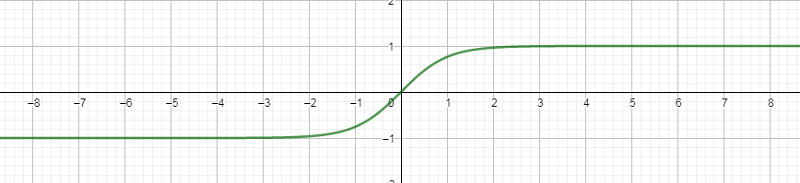
\includegraphics[width=\textwidth]{tanh.png}

\vspace{5}
Here notice that if $z$ takes on only a small range of parameters, that is $|z|$ is close to zero, then you're just using the linear regime of the $tanh$ function. If only if $z$ is allowed to wander up to larger values or smaller values or $|z|$ is farther from 0, that the activation function starts to become less linear. So the intuition you might take away from this is that if $\lambda$, the regularization parameter, is large, then you have that your parameters will be relatively small, because they are penalized being large into a cost function.

And so if the weights of $w$ are small then because $z = wx+b4$ but if $w$ tends to be very small, then $z$ will also be relatively small. And in particular, if $z$ ends up taking relatively small values, it would cause of $g(z)$ to roughly be linear. So it is as if every layer will be roughly linear like linear regression. This would make it just like a linear network. And so even a very deep network, with a linear activation function is at the end only able to compute a linear function. This would not make it possible to fit some very complicated decisions.

If you have a neural net and some very complicated decisions you could possibly overfit and this could definitely help reducing your overfitting.


\maketitle
\section{A tip to remember}

When  you implement gradient descent, one of the steps to debug gradient descent is to plot the cost function $J$ as a function of the number of elevations of gradient descent and you want to see that the cost function $J$ decreases monotonically after every elevation of gradient descent. And if you're implementing regularization then remember that $J$ now has a new definition. If you plot the old definition of $J$, then you might not see a decrease monotonically. So, to debug gradient descent make sure that you're plotting this new definition of $J$ that includes this second term as well. Otherwise you might not see $J$ decrease monotonically on every single elevation.

I have found regularization pretty helpful in my Deep Learning models and have helped me solve overfitting quite a few times, I hope they can help you too.

\maketitle
\section{About Me}

Hi everyone I am Rishit Dagli
LinkedIn - linkedin.com/in/rishit-dagli-440113165/
Website - rishit.tech
If you want to ask me some questions, report any mistake, suggest improvements, give feedback you are free to do so by mailing me at - 
rishit.dagli@gmail.com
hello@rishit.tech

\end{document}
